\documentclass[journal,12pt,twocolumn]{IEEEtran}

\usepackage{setspace}
\usepackage{gensymb}

\singlespacing 



\usepackage[cmex10]{amsmath}

\usepackage{amsthm}

\usepackage{mathrsfs}
\usepackage{txfonts}
\usepackage{stfloats}
\usepackage{bm}
\usepackage{cite}
\usepackage{cases}
\usepackage{subfig}

\usepackage{longtable}
\usepackage{multirow}

\usepackage{enumitem}
\usepackage{mathtools}
\usepackage{steinmetz}
\usepackage{tikz}
\usepackage{circuitikz}
\usepackage{verbatim}
\usepackage{tfrupee}
\usepackage[breaklinks=true]{hyperref}
\usepackage{graphicx}
\usepackage{tkz-euclide}
\usepackage{float}

\usetikzlibrary{calc,math}
\usepackage{listings}
    \usepackage{color} %%
    \usepackage{array} %%
    \usepackage{longtable} %%
    \usepackage{calc} %%
    \usepackage{multirow} %%
    \usepackage{hhline} %%
    \usepackage{ifthen} %%
    \usepackage{lscape}     
\usepackage{multicol}
\usepackage{chngcntr}
\newcommand{\norm}[1]{\left\lVert#1\right\rVert}

\DeclareMathOperator*{\Res}{Res}

\renewcommand\thesection{\arabic{section}}
\renewcommand\thesubsection{\thesection.\arabic{subsection}}
\renewcommand\thesubsubsection{\thesubsection.\arabic{subsubsection}}

\renewcommand\thesectiondis{\arabic{section}}
\renewcommand\thesubsectiondis{\thesectiondis.\arabic{subsection}}
\renewcommand\thesubsubsectiondis{\thesubsectiondis.\arabic{subsubsection}}


\hyphenation{op-tical net-works semi-conduc-tor}
\def\inputGnumericTable{} %%

\lstset{
%language=C,
frame=single, 
breaklines=true,
columns=fullflexible
}
\begin{document}


\newtheorem{theorem}{Theorem}[section]
\newtheorem{problem}{Problem}
\newtheorem{proposition}{Proposition}[section]
\newtheorem{lemma}{Lemma}[section]
\newtheorem{corollary}[theorem]{Corollary}
\newtheorem{example}{Example}[section]
\newtheorem{definition}[problem]{Definition}

\newcommand{\BEQA}{\begin{eqnarray}}
\newcommand{\EEQA}{\end{eqnarray}}
\newcommand{\define}{\stackrel{\triangle}{=}}
\newcommand\hlight[1]{\tikz[overlay, remember picture,baseline=-\the\dimexpr\fontdimen22\textfont2\relax]\node[rectangle,fill=blue!50,rounded corners,fill opacity = 0.2,draw,thick,text opacity =1] {$#1$};}
\bibliographystyle{IEEEtran}
\providecommand{\mbf}{\mathbf}
\providecommand{\pr}[1]{\ensuremath{\Pr\left(#1\right)}}
\providecommand{\qfunc}[1]{\ensuremath{Q\left(#1\right)}}
\providecommand{\sbrak}[1]{\ensuremath{{}\left[#1\right]}}
\providecommand{\lsbrak}[1]{\ensuremath{{}\left[#1\right.}}
\providecommand{\rsbrak}[1]{\ensuremath{{}\left.#1\right]}}
\providecommand{\brak}[1]{\ensuremath{\left(#1\right)}}
\providecommand{\lbrak}[1]{\ensuremath{\left(#1\right.}}
\providecommand{\rbrak}[1]{\ensuremath{\left.#1\right)}}
\providecommand{\cbrak}[1]{\ensuremath{\left\{#1\right\}}}
\providecommand{\lcbrak}[1]{\ensuremath{\left\{#1\right.}}
\providecommand{\rcbrak}[1]{\ensuremath{\left.#1\right\}}}
\theoremstyle{remark}
\newtheorem{rem}{Remark}
\newcommand{\sgn}{\mathop{\mathrm{sgn}}}
%\providecommand{\abs}[1]{\left\vert#1\right\vert}
\providecommand{\res}[1]{\Res\displaylimits_{#1}} 
\providecommand{\norm}[1]{$\left\lVert#1\right\rVert$}
%\providecommand{\norm}[1]{\lVert#1\rVert}
\providecommand{\mtx}[1]{\mathbf{#1}}
%\providecommand{\mean}[1]{E\left[ #1 \right]}
\providecommand{\fourier}{\overset{\mathcal{F}}{ \rightleftharpoons}}
%\providecommand{\hilbert}{\overset{\mathcal{H}}{ \rightleftharpoons}}
\providecommand{\system}{\overset{\mathcal{H}}{ \longleftrightarrow}}
 %\newcommand{\solution}[2]{\textbf{Solution:}{#1}}
\newcommand{\solution}{\noindent \textbf{Solution: }}
\newcommand{\cosec}{\,\text{cosec}\,}
\providecommand{\dec}[2]{\ensuremath{\overset{#1}{\underset{#2}{\gtrless}}}}
\newcommand{\myvec}[1]{\ensuremath{\begin{pmatrix}#1\end{pmatrix}}}
\newcommand{\mydet}[1]{\ensuremath{\begin{vmatrix}#1\end{vmatrix}}}
\numberwithin{equation}{subsection}
\makeatletter
\@addtoreset{figure}{problem}
\makeatother
\let\StandardTheFigure\thefigure
\let\vec\mathbf
\renewcommand{\thefigure}{\theproblem}
\def\putbox#1#2#3{\makebox[0in][l]{\makebox[#1][l]{}\raisebox{\baselineskip}[0in][0in]{\raisebox{#2}[0in][0in]{#3}}}}
     \def\rightbox#1{\makebox[0in][r]{#1}}
     \def\centbox#1{\makebox[0in]{#1}}
     \def\topbox#1{\raisebox{-\baselineskip}[0in][0in]{#1}}
     \def\midbox#1{\raisebox{-0.5\baselineskip}[0in][0in]{#1}}
\vspace{3cm}
\title{Assignment No.5}
\author{Sravani sandya}
\maketitle
\newpage
\bigskip
\renewcommand{\thefigure}{\theenumi}
\renewcommand{\thetable}{\theenumi}
Download latex-tikz codes from
\begin{lstlisting}
https://github.com/sravani706/Assignment5/main/main.tex
\end{lstlisting}
%
Download python codes from
\begin{lstlisting}
https://github.com/sravani706/Assignment5/main/main.tex
\end{lstlisting}
%
Question taken from
\begin{lstlisting}
Quadratic_forms, exercise 2
\end{lstlisting}
\section{Question No 2.30}
Find the equation of the hyperbola with vertices
\myvec{0 \\\pm\frac{\sqrt{11}}{2}} and foci are \myvec{0 \\\pm 3}
\section{Solution}
We have been provided with values for vertices and foci
\newline
The given vertices are- \myvec{0 \\\pm\frac{\sqrt{11}}{2}}
\newline
The given vertices are in the form of \myvec{0 \\\pm 3}
Here, The major axis is along X axis
\newline
The equation of conic is given as 
\begin{align}
\vec{u}^T(\vec{t}^T-\vec{nn}^T) \vec{u}+2(\vec{cn}-\vec{tf}^T\vec{u}+\vec{t}\norm{F}^2-\vec{c}^2=0
\end{align}
Thus,
\begin{align}
\vec{F}=\myvec{0\\\pm 3}, \vec{n}= \myvec{0\\1},\vec{c}=0, \vec{t}=\frac{1}{9}
\end{align}
\begin{align}\label{eq:1}
\vec{n}^T\brak{\frac{1}{9}\myvec{1\ 0\\ 0\ 1}-\myvec{0\\1}\myvec{0\ 1}}\vec{u}+2\brak{0-\frac{1}{9}\myvec{0\\\pm3}}^T\vec{u}+\frac{1}{9}\norm{\myvec{0\\\pm3}}^2-0=0
\end{align}
\begin{align}
\vec{u}^T\brak{\myvec{\frac{-8}{9}\ 0 \\ 0\ \frac{-8}{9}}}\vec{u}+2\myvec{0 \ \frac{1}{3}}\vec{u}+1=0
\end{align}
Replacing \vec{u} by \myvec{u \\ v} in \eqref{eq:1}
\begin{align}
\frac{\vec{u}^2}{\frac{9}{8}}+\frac{\vec{v}^2}{\frac{9}{8}}+\frac{2}{3}\vec{v}=1
\end{align}
\begin{align}
\frac{8}{9}\vec{u}^2+\frac{8}{9}\vec{v}^2+\frac{2}{3}\vec{v}=1
\end{align}
\begin{align}
 8\vec{u}^2+8\vec{v}^2+6\vec{v}=9\\
\end{align}
$\therefore$ this is the equation of hyperbola 
\begin{figure}[ht]
\centering
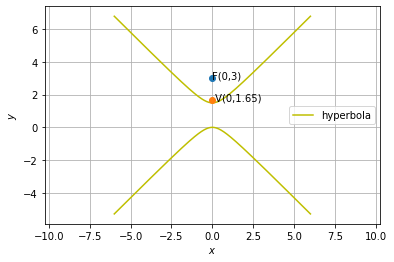
\includegraphics[width=\columnwidth]{download.png}
\caption{Hyperbola}
\label{Hyperbola along given axis}
\end{figure}
\end{document}
